% =====================================================================
\section{ODMR physics and line shapes}
\label{sm:odmr}
% =====================================================================

This section gives the physics behind the line model of Sec.~\ref{sec:model} of the main text: the optical
readout of the N-V spin, the Rabi response that sets the CW and pulsed line shapes, the hyperfine structure and the
second transition that Eq.~\eqref{eq:signal} leaves out, and the derivation of the line shapes with the laser
treated as two rates rather than a reset, the broadening by the spin bath, and the pulsed readout.

\subsection{Optical readout}

The negatively charged N-V center is described by five levels
\cite{manson2006,doherty2013nv} (Fig.~\ref{fig:levels}): the spin-triplet ground state $^3A_2$, split into
$|0\rangle_g$ and $|\pm1\rangle_g$ by the spin projection $m_s$ on the N-V axis; the spin-triplet excited state
$^3E$, with $|0\rangle_e$ and $|\pm1\rangle_e$; and a metastable spin singlet $|s\rangle$ that stands for the
singlet manifold. Green light drives the spin-conserving optical transitions $|m_s\rangle_g\to|m_s\rangle_e$, which
decay back by emitting red photoluminescence (PL). From $|\pm1\rangle_e$, however, the intersystem crossing to the
singlet is much faster than from $|0\rangle_e$, and the singlet decays preferentially to $|0\rangle_g$.
% The singlet -> |g,0> branching ratio is still debated: ~50-70 % (Robledo et al. 2011; Tetienne et al. 2012)
% vs ~90 % (Wirtitsch et al.), as summarized in arXiv:2511.19583. Not needed here: only the net pumping into
% m_s = 0 enters, through the rate Gamma_p below. Verify the primary sources before quoting a number.
Two
consequences follow. Under continuous illumination the spin is pumped into $m_s=0$; and a center in $m_s=\pm1$
spends part of its optical cycles in the dark singlet, so it emits less PL than one in $m_s=0$. The spin state can
therefore be prepared and read out optically.
\begin{figure}[t]
\centering
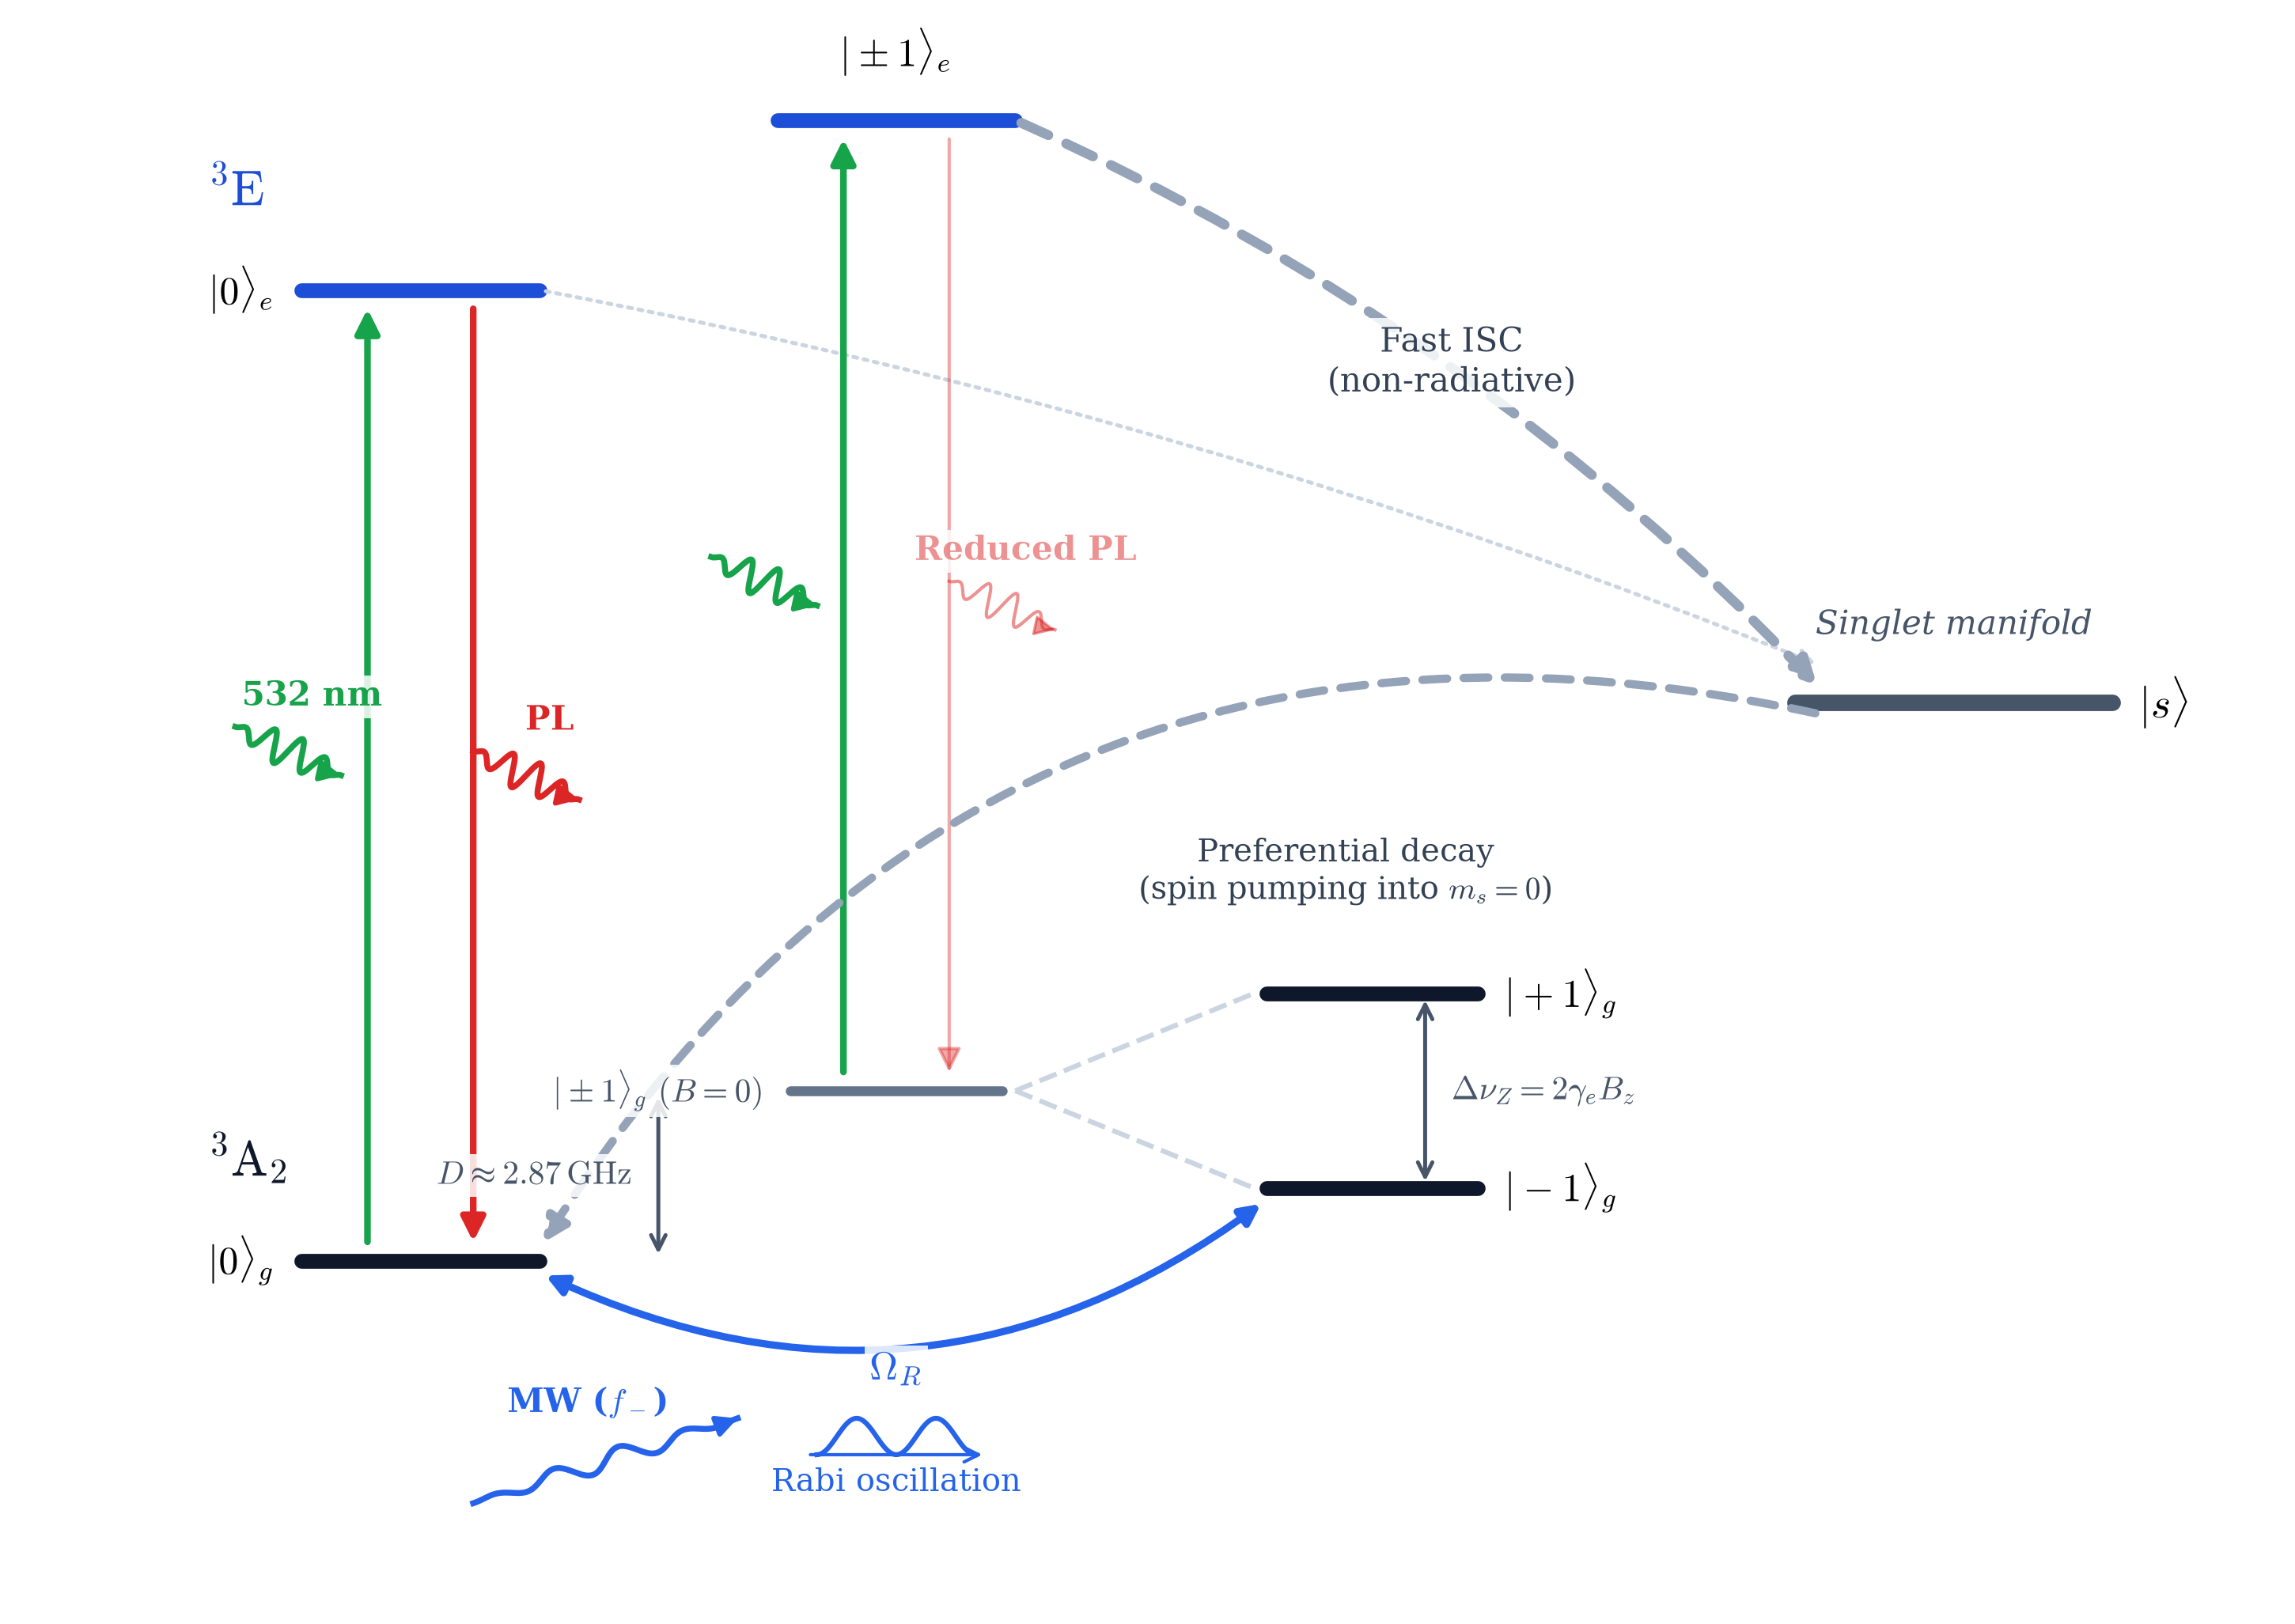
\includegraphics[width=\linewidth]{nv_5level_diagram}
\caption{Five-level model of the N-V center \cite{manson2006,doherty2013nv}. \tbd{Caption to follow the figure.}}
\label{fig:levels}
\end{figure}

The two transitions $f_\pm$ share the state $|0\rangle_g$ but lie $2\delta_Z$ apart. When this separation is large
compared with the linewidth, a drive near $f_-$ is far off resonance with $f_+$ and couples only $|0\rangle_g$ and
$|-1\rangle_g$. The excited state and the singlet then enter only through the rates at which the laser repolarizes
the spin and destroys its coherence \cite{dreau2011}, so the spin reduces to a driven two-level system
$\{m_s=0,m_s=-1\}$.

\subsection{Rabi response and the two ODMR modes}

Let the drive have detuning $\Delta=f-f_-$ from the transition and Rabi frequency $\Omega$, the rate in Hz at which
the population oscillates on resonance. Off resonance the spin oscillates faster but less deeply, at the
generalized Rabi frequency
\begin{equation*}
  \Omega_{\rm gen}=\sqrt{\Omega^2+\Delta^2}.
\end{equation*}
Starting from $m_s=0$, the probability of finding the spin in $m_s=-1$ after a drive of duration $t$ is
\begin{equation}
  P_{-1}(\Delta,t)=\frac{\Omega^2}{\Omega_{\rm gen}^2}\,\sin^2\!\big(\pi\Omega_{\rm gen} t\big),
  \label{eq:rabi}
\end{equation}
and $P_0=1-P_{-1}$ is the probability of finding it still in $m_s=0$. The prefactor is the depth of the
oscillation, the sine its time dependence. Since $m_s=-1$ is the darker state, the PL dip is proportional to
$P_{-1}$. How the drive is applied sets the line shape.
\begin{figure}[t]
\centering
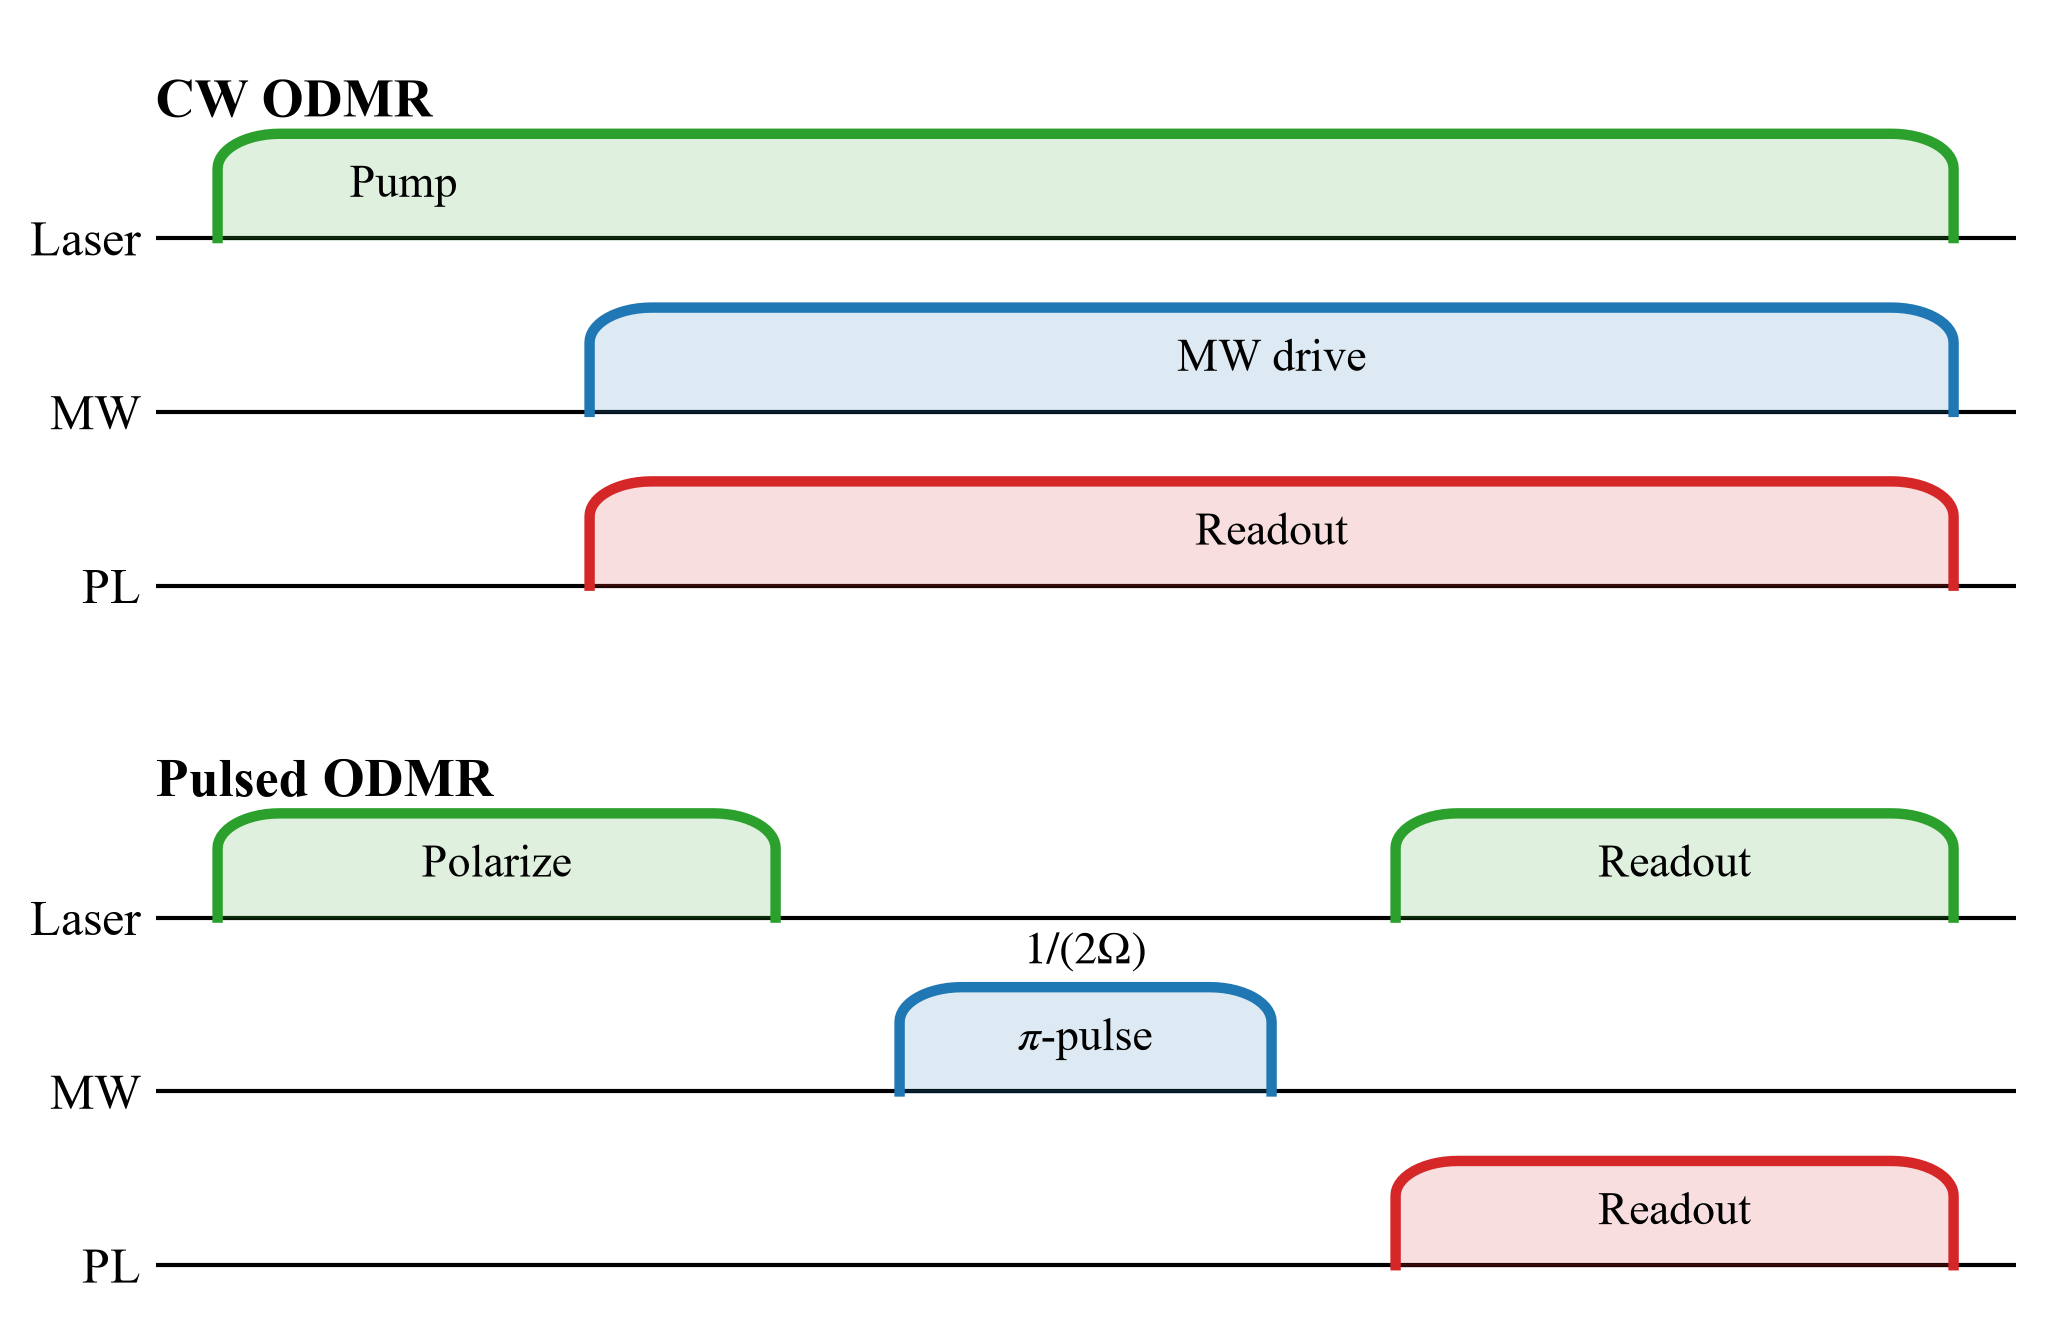
\includegraphics[width=\linewidth]{odmr_sequence}
\caption{Laser and microwave sequences of CW and pulsed ODMR. \tbd{Caption to follow the figure.}}
\label{fig:sequences}
\end{figure}

\paragraph{CW ODMR.} In continuous-wave ODMR the laser and the microwave drive act on the spin continuously and at the
same time, and the PL is read out while the drive is on (Fig.~\ref{fig:sequences}). The laser keeps pumping the spin
back into $m_s=0$ while the drive keeps rotating it away, so every optical reset starts a new Rabi oscillation, and
the PL, collected over many such cycles, reports Eq.~\eqref{eq:rabi} averaged over the time $T$ between resets.
When the drive acts for many Rabi periods between resets, $\Omega_{\rm gen} T\gg1$, the oscillating factor averages to
$\tfrac12$,
\begin{equation}
  \bar P_{-1}(\Delta)=\frac{\Omega^2}{\Omega_{\rm gen}^2}\,\frac1T\int_0^T\sin^2\!\big(\pi\Omega_{\rm gen} t\big)\,dt
  \;\longrightarrow\;\frac12\,\frac{\Omega^2}{\Omega^2+\Delta^2}.
  \label{eq:cw-lorentzian}
\end{equation}
The average only renormalizes the amplitude; the line shape is that of the prefactor, a Lorentzian in the detuning
$\Delta$ of half width $\Omega$. This is the microwave contribution to the width, power broadening: the stronger the
drive, the further off resonance it still flips the spin. With the laser treated as two rates rather than a reset
(Sec.~\ref{sm:cw-pumping}), the line stays a Lorentzian, with the half width of Eq.~\eqref{eq:linewidth} of the
main text.

\paragraph{Pulsed ODMR} is a technique that removes the laser from the width of the line \cite{dreau2011}. In CW ODMR the
laser that reads the spin out also broadens the line through $\Gamma_c$, and narrowing it means lowering both powers
and with them the contrast and the PL. Pulsed ODMR separates the two in time: a laser pulse polarizes the spin into
$m_s=0$, the laser is switched off while a single microwave $\pi$-pulse of duration $t_\pi=1/(2\Omega)$ is applied,
and a second laser pulse reads the spin out (Fig.~\ref{fig:sequences}). The pulse fully inverts the spin on
resonance, and Eq.~\eqref{eq:rabi} at $t=t_\pi$ gives (Sec.~\ref{sm:pulsed})
\begin{equation}
  P_{-1}^{\pi}(\Delta)=\frac{\Omega^2}{\Omega_{\rm gen}^2}\,\sin^2\!\Big(\frac{\pi}{2}\,\frac{\Omega_{\rm gen}}{\Omega}\Big).
  \label{eq:pulsed}
\end{equation}
This line is not a Lorentzian. Its width is the Fourier limit of the pulse, $\sim1/t_\pi$, down to $\sim1/T_2^*$,
where the spread of the transition frequency sets it, and it has side lobes up to 12\% of the depth: dips where there
is no resonance, a hazard for a search.

% Code: NVCenterPulsedDriveModel (spectra/nv_center_drive.py) evaluates Eq. (rabi) at the pulse time with the
% Gaussian T2* average; NVCenterCWDriveModel broadens with MW power only, gamma = gamma_0 sqrt(1 + s_MW),
% gamma_0 = 150 kHz fixed, i.e. no optical term. The SNR x window study uses a fixed linewidth (no drive),
% consistent with one Gamma.

\subsection{Terms left out of the line model}

The Hamiltonian of Eq.~\eqref{eq:hamiltonian} drops the strain term $E(S_x^2-S_y^2)$, since it is a small correction
when $\gamma_e B_z\gg E$.

Each nuclear projection $m_I$ gives its own copy of the line, shifted by
$A_\parallel m_I$ (Eq.~\eqref{eq:transitions}) and weighted by the population of that $m_I$, so the observed
spectrum is a sum of $2I+1$ lines. Two cases reduce it to the single line of Eq.~\eqref{eq:signal}. Near the
excited-state level anticrossing the nitrogen nuclear spin is polarized into a single $m_I$ \cite{jacques2009}: only
one line remains, and its fixed offset $A_\parallel m_I$ is absorbed into $f_-$. When the line is much wider than
the hyperfine spacing, $\Gamma\gg|A_\parallel|$, the lines merge into one.

Equation~\eqref{eq:signal} also leaves out the $f_+$ line. The drive window lies below $D$ and holds $f_-$ only, but
the tail of the $f_+$ line, $2\delta_Z$ higher, adds $C\gamma^2/[\gamma^2+(f-f_+)^2]$ inside it: at $f_-$ a fraction
$\gamma^2/(\gamma^2+4\delta_Z^2)$ of the contrast $C$, i.e.\ 20\% at $\delta_Z=\gamma$ and below 1\% for
$\delta_Z\gtrsim5\gamma$. Equation~\eqref{eq:signal} assumes $\delta_Z\gg\gamma$; small Zeeman shifts, where the two
lines overlap, are outside the scope of this work. The same tail raises the on-resonance depth to
$C[1+\gamma^2/(\gamma^2+4\delta_Z^2)]$, so the SNR $C/\sigma$ of Eq.~\eqref{eq:snr} is the $\delta_Z\gg\gamma$ limit
of the on-resonance SNR.

\subsection{CW line with optical pumping}
\label{sm:cw-pumping}

Eq.~\eqref{eq:cw-lorentzian} treats the laser only as a reset, which is too
crude when the resets are frequent. The laser acts on the spin through two rates, both set by how often the center
goes through an optical cycle: it pumps the spin back toward $m_s=0$, at a rate $\Gamma_p$, and each cycle destroys
the phase between $m_s=0$ and $m_s=-1$, at a rate $\Gamma_c$. The two rates share a cause but are not equal. A cycle
that excites the center destroys the phase whatever happens next, since in the excited state the spin evolves under
a different Hamiltonian and the decay path records its state; only the cycles that pass through the singlet move
population into $m_s=0$. Every pumping cycle therefore destroys the phase, but not every phase-destroying cycle
pumps, and $\Gamma_c$ exceeds $\Gamma_p$.
% The ordering Gamma_c > Gamma_p follows Dreau et al. (2011), whose saturated values differ by about an order of
% magnitude. Verify the values there before quoting numbers.
The spin's environment adds rates of its own, independent of the laser: its longitudinal relaxation $1/T_1$ adds
to $\Gamma_p$ and its homogeneous dephasing $1/T_2$ adds to $\Gamma_c$, giving the total rates
$\Gamma_1=\Gamma_p+1/T_1$ for the populations and $\Gamma_2=\Gamma_c+1/T_2$ for the coherence of
Eq.~\eqref{eq:linewidth}. At the laser powers of CW ODMR both environmental rates are slow against the optical ones,
$\Gamma_1\approx\Gamma_p$ and $\Gamma_2\approx\Gamma_c$, but the derivation below holds for any values of the totals.
The slow spread of the transition frequency, which sets $T_2^*$, is not a rate of this kind and is treated
separately below. The microwave enters only through its angular Rabi
frequency $\Omega_R=2\pi\Omega$. The competition between the two is clearest in terms of populations. A drive whose
coherence is destroyed at the rate $\Gamma_2$ no longer produces Rabi oscillations; it moves population between
$m_s=0$ and $m_s=-1$, in both directions alike, at the rate
\begin{equation}
  W(\Delta)=\frac{\Omega_R^2\,\Gamma_2}{2\big[\Gamma_2^2+(2\pi\Delta)^2\big]}
  =\frac{\Omega_R^2}{2\Gamma_2}\,\frac{\Gamma_2^2}{\Gamma_2^2+(2\pi\Delta)^2},
  \label{eq:transfer-rate}
\end{equation}
a Lorentzian of peak $\Omega_R^2/2\Gamma_2$ and half width $\Gamma_2/2\pi$ in Hz. The laser, helped by $T_1$, returns
population from $m_s=-1$ at the rate $\Gamma_1$, so with $P_0=1-P_{-1}$ the population of $m_s=-1$ obeys
\begin{equation*}
  \dot P_{-1}=W\,(P_0-P_{-1})-\Gamma_1P_{-1}=W-(2W+\Gamma_1)\,P_{-1}.
\end{equation*}
In steady state, inserting Eq.~\eqref{eq:transfer-rate} and then ordering the terms of the denominator,
\begin{equation}
  \begin{aligned}
  P_{-1}^{\rm ss}(\Delta)&=\frac{W}{2W+\Gamma_1}
  =\frac12\,\frac{\Omega_R^2\,\Gamma_2}{\Omega_R^2\,\Gamma_2+\Gamma_1\big[\Gamma_2^2+(2\pi\Delta)^2\big]}\\
  &=\frac12\,\frac{\Omega_R^2\,\Gamma_2/\Gamma_1}{(2\pi\Delta)^2+\Gamma_2^2+\Omega_R^2\,\Gamma_2/\Gamma_1},
  \end{aligned}
  \label{eq:bloch-ss}
\end{equation}
the same as the steady state of the full Bloch equations \cite{dreau2011}. It reduces to
Eq.~\eqref{eq:cw-lorentzian} when the two rates are equal and small against $\Omega_R$. The last form is a
Lorentzian in $2\pi\Delta$ whose squared half width is the constant in its denominator, which gives
Eq.~\eqref{eq:linewidth}.

The first term of Eq.~\eqref{eq:linewidth} is the width without drive, set by the loss of coherence. The
second is power broadening by the microwave: a strong drive saturates the transfer, $W\gg\Gamma_1$, already on the
tails of the line, and the line widens until $W$ there has fallen to about the pumping rate. The depth of the line,
Eq.~\eqref{eq:bloch-ss} at $\Delta=0$, is
\begin{equation*}
  P_{-1}^{\rm ss}(0)=\frac12\,\frac{\Omega_R^2}{\Omega_R^2+\Gamma_1\Gamma_2}:
\end{equation*}
it grows with the microwave power, toward $\tfrac12$, and falls with the laser power, which repolarizes the spin
before the drive can flip it.

\paragraph{Optical saturation.} The two laser rates grow with the laser power, but not without limit. The optical
transition is itself a two-level system: the laser excites the center at a rate proportional to its intensity
$I_{\rm opt}$, and the excited state decays in its lifetime $\tau_e$. In steady state the excited population is
$s/(1+s)$, with the saturation parameter $s=I_{\rm opt}/I_{\rm sat}$ the ratio of the excitation rate to the decay
rate $1/\tau_e$. At low power it grows linearly with $s$; at high power it levels off, because a center cannot be
excited again before it has decayed. The rate of optical cycles is this population divided by $\tau_e$, and both
laser rates follow it, $\Gamma_{p,c}=\Gamma_{p,c}^\infty\,s/(1+s)$ \cite{dreau2011}, with $\Gamma_{p,c}^\infty$ their
values at full saturation. Raising the laser power therefore both widens and flattens the line, up to saturation.
% Dreau et al. (2011) Eq. 11 quotes the same width as Gamma_c^inf/(2 pi) sqrt((s/(1+s))^2 + Omega_R^2/(Gamma_p^inf
% Gamma_c^inf)) and calls it the FWHM; with Gamma_{p,c} = Gamma^inf s/(1+s) this is Eq. (linewidth) up to their
% factor-2 convention for the rates. Check before quoting numbers.

\paragraph{Spin bath in the CW line.} The local fields of the spin bath, mostly the $^{13}$C nuclear spins, shift
the transition by a random offset $\xi$ that changes slowly, over times much longer than the repolarization time
$1/\Gamma_p$. The spin therefore reaches the steady state of Eq.~\eqref{eq:bloch-ss} at the detuning $\Delta-\xi$
before $\xi$ changes, and a measurement that averages over many values of $\xi$ records that steady state convolved
with their distribution, the same average as Eq.~\eqref{eq:pulsed-t2star} below. For a Gaussian distribution of
standard deviation $\sigma_\xi=1/(\sqrt2\,\pi T_2^*)$ the CW line is a Voigt profile: the Lorentzian of
Eq.~\eqref{eq:bloch-ss}, of half width $\gamma$, convolved with a Gaussian of width $\sigma_\xi$. When
$\gamma\gg\sigma_\xi$ it is the Lorentzian of Eq.~\eqref{eq:signal}; when the laser and microwave powers are
lowered until $\gamma\lesssim\sigma_\xi$, the line stops narrowing at a width $\sim1/T_2^*$, as the pulsed line does.
In either case it is one dip with one total width, which is the width inferred in Sec.~\ref{sec:methods} of the main
text; the simulations use a pseudo-Voigt approximation to this profile.

\subsection{Pulsed line}
\label{sm:pulsed}

The $\pi$-pulse length is chosen so that on resonance, where the spin oscillates at
$\Omega$, it is fully inverted: $\pi\Omega t_\pi=\pi/2$. Off resonance it oscillates at $\Omega_{\rm gen}$ instead, so
the argument of the sine in Eq.~\eqref{eq:rabi} at $t=t_\pi$ is $\pi\Omega_{\rm gen} t_\pi=(\pi/2)\,\Omega_{\rm gen}/\Omega$,
which gives Eq.~\eqref{eq:pulsed}. On resonance $\Omega_{\rm gen}=\Omega$ and the inversion is complete. For
$|\Delta|\gg\Omega$, $\Omega_{\rm gen}\approx|\Delta|$ and
$P_{-1}^{\pi}\approx\sin^2(\pi\Delta t_\pi)/(2\Delta t_\pi)^2$, the power spectrum of a rectangular pulse of length
$t_\pi$: far from resonance the spin responds to the frequency content of the pulse. The line vanishes wherever
$\Omega_{\rm gen}=2\Omega,4\Omega,\dots$, i.e.\ at $|\Delta|=\sqrt3\,\Omega,\sqrt{15}\,\Omega,\dots$: there the spin
completes a whole number of full Rabi cycles during the pulse and returns to $m_s=0$. Between the zeros lie side
lobes that decay as $\Omega^2/\Omega_{\rm gen}^2$; the first, near $\Omega_{\rm gen}=3\Omega$ at $|\Delta|\approx2.7\,\Omega$,
is 12\% of the depth.

\paragraph{Inhomogeneous broadening.} The transition frequency of the spin is not sharp: slowly fluctuating local
fields, mostly from the bath of $^{13}$C nuclear spins, shift it by a random offset $\xi$ that is fixed during one
pulse but changes from one repetition of the sequence to the next. A measurement averages many repetitions, each
driven at the detuning $\Delta-\xi$ instead of $\Delta$, so the measured line is Eq.~\eqref{eq:pulsed} averaged over
the distribution of $\xi$, i.e.\ convolved with it. For a Gaussian distribution of standard deviation $\sigma_\xi$,
\begin{equation}
  \bar P_{-1}^{\pi}(\Delta)=\int P_{-1}^{\pi}(\Delta-\xi)\,\frac{e^{-\xi^2/2\sigma_\xi^2}}{\sqrt{2\pi}\,\sigma_\xi}\,d\xi .
  \label{eq:pulsed-t2star}
\end{equation}
The width $\sigma_\xi$ is what $T_2^*$ measures. A free spin precessing at the offset $\xi$ picks up the phase
$2\pi\xi t$, and the average of $e^{2\pi i\xi t}$ over the Gaussian is the coherence envelope
$e^{-2\pi^2\sigma_\xi^2t^2}$. $T_2^*$ is defined by writing this envelope as $e^{-(t/T_2^*)^2}$, so
$\sigma_\xi=1/(\sqrt2\,\pi T_2^*)$. For $t_\pi\ll T_2^*$ the spread is small against $\Omega$ and the line is that of
Eq.~\eqref{eq:pulsed}. For $t_\pi\gtrsim T_2^*$ the Gaussian dominates: the zeros and side lobes are washed out, the
line stops narrowing at a width $\sim1/T_2^*$, and the depth falls because the pulse no longer inverts every
frequency class \cite{dreau2011}.

\paragraph{Readout.} While the microwave pulse is on, the laser is off and the spin relaxes only through $T_1$, which
is much longer than $t_\pi$, and dephases through the spread already included in Eq.~\eqref{eq:pulsed-t2star}. The
readout is different: the laser that reads the spin out also repolarizes it, so the PL difference between $m_s=0$
and $m_s=-1$ lasts only for the repolarization time $\tau_p$. Taking the repolarization as a single exponential, a
spin flipped with probability $P_{-1}$ emits, a time $t$ into the readout pulse, PL at the rate
$\Phi_0\,[1-c\,P_{-1}\,e^{-t/\tau_p}]$, where $\Phi_0$ is the rate of $m_s=0$ and $c$ the fractional PL drop of
$m_s=-1$ at the start of the readout. The recorded PL is this rate integrated over a readout window of length $t_r$,
normalized to the same integral with no flip,
\begin{equation}
  \begin{aligned}
  \mu&=1-\frac{1}{t_r}\int_0^{t_r}c\,P_{-1}\,e^{-t/\tau_p}\,dt\\
  &=1-c\,\frac{\tau_p}{t_r}\big(1-e^{-t_r/\tau_p}\big)\,\bar P_{-1}^{\pi}(\Delta) ,
  \end{aligned}
  \label{eq:pulsed-readout}
\end{equation}
with $P_{-1}=\bar P_{-1}^{\pi}$ of Eq.~\eqref{eq:pulsed-t2star}. The integration leaves the line shape unchanged and
sets only its depth: the contrast is $C=c\,(\tau_p/t_r)(1-e^{-t_r/\tau_p})$. A longer window collects more photons,
$N_{\rm ph}\propto t_r$, but dilutes the contrast, so the single-shot signal-to-noise ratio
$C\sqrt{N_{\rm ph}}\propto(1-e^{-t_r/\tau_p})/\sqrt{t_r/\tau_p}$ is largest at $t_r\approx1.26\,\tau_p$.
